\clearpage
\section{QCD $\times$ dark QCD} \label{QCDxdQCD}
  
  Das Verhalten der QCD-Kopplungskonstanten ist im Standardmodell allein nicht 
  im Stande ein asymptotic safety Szenario zu entwickeln, wie in Abschnitt 
  \ref{beta_im_SM} gezeigt wird. Durch die 
  Erweiterung der QCD um eine weitere Eichgruppe, die dark QCD, ergeben sich 
  qualitativ völlig neue Möglichkeiten im Hochenergieverhalten der 
  Kopplungskonstanten. 
  
  \subsection{Die Standardmodell QCD}
    Im Standardmodell wird die QCD durch die Symmetriegruppe $SU(\Nc)$ 
    dargestellt, unter der sich die Quarks in der 
    \textit{fundamentalen Darstellung} und die Gluonen in der 
    \textit{adjungierten Darstellung} transformieren. Im SM gibt es 
    $N_\text{Flavour}=6$
    verschiedene Quarkflavour und $N_\text{Colour}=3$ Colours, da die QCD 
    Flavour-Blind ist, d.h. da die Wechselwirkung unabhängig von der 
    Flavour-Quantenzahl ist, ist die 
    Erweiterung auf $\Nc$ Colour und $\nfc$ Flavour jedoch trivial. Die 
    Lagrangedichte kann als 
    \begin{equation}
     \mathcal{L}_\text{QCD} =\bar{\psi}_i^f \left( 
     \i \gamma^\mu \partial_\mu \delta_{ij} 
     -g_1 \gamma^\mu t^A_{ij} \mathcal{A}_\mu^A
     -m_f \delta_{ij}
     \right)\psi_j^f -\frac{1}{4} F_{\mu \nu}^A F^{A \,\,\, \mu\nu}
     \label{eq:QCDxdQCD:L_QCD}
    \end{equation}
    geschrieben werden \cite{PDG:QCD}. Dabei stellt $\psi_b^f$ ein Quarkfeld mit 
    Colour $i$ und Flavour $f\in\{1,2,\ldots,\nfc\}$ 
    und mit der Masse 
    $m_f$ dar, $g_1$ ist die Kopplungskonstante der QCD. Die Indizes $i,j\in
    \{1,2,\ldots \Nc\}$ gehören zur fundamentalen Darstellung, während $A\in 
    \{1,2,\dots,\Nc^2-1\}$ zur adjungierten Darstellung gehört. Man 
    nennt $\psi=(\psi_1,\psi_2,\ldots,\psi_{\Nc})^\text{T}$ ein 
    Colour-Multiplett\footnote{Der Flavour-Index $f$ wird ab jetzt 
    weggelassen.} unter der fundamentalen Darstellung, wenn es unter 
    Anwendung der $SU(\Nc)$ gemäß
    \begin{equation}
      \psi(x) \longrightarrow \underbrace{U(x)}_{\in \mathbb{C}^{\Nc\times\Nc}}
      \psi(x) \quad ,\quad \bar{\psi}(x) \longrightarrow\bar{\psi}(x) 
      U(x)^\dagger
    \end{equation}
    transformiert. Die Gluonfelder $\mathcal{A}_\mu^A$ mit Erzeugern 
    $t^A\in \mathbb{C}^{\Nc\times\Nc}$ 
    transformieren dagegen in der 
    adjungierten Darstellung \cite{Weinberg:QFT_2}
    \begin{equation}
      t^A_{ij}\mathcal{A}_\mu^A(x) \longrightarrow
      U(x) t^A_{ij}\mathcal{A}_\mu^C(x) U(x)^\dagger - \i (\partial_\mu U(x) )
      U(x)^\dagger \quad .
    \end{equation}
    Die Dynamik und Propagation der Gluonen wird dabei durch den 
    Feldstärketensor vermittelt,
    \begin{equation}
      F^A_{\mu\nu} = \partial_\mu \mathcal{A}_\nu^A-\partial_\nu 
      \mathcal{A}_\mu^A - g f^{ABC} \mathcal{A}_\mu^B \mathcal{A}_\nu^C 
      \quad , \quad [t^A,t^B]=\i f^{ABC} t^C  \quad .
      \label{eq:QCDxdQCD:Feldstaerketensor}
    \end{equation}
    Versucht man die QCD im Feynmanformalismus zu quantisieren, werden außerdem 
    Eichfixierung und Faddeev-Popov-de-Witt Ghosts benötigt  
    \cite{Weinberg:QFT_2}, diese können jedoch nach der Modellbildung 
    hinzugefügt werden, sodass sie hier nicht auftauchen. 
    
    %DIAGRAMME
    
  \subsection{Dark QCD}
    In \cite{Scale_of_dark_QCD} wird die dQCD eingeführt, um die DM Massendichte 
    $\Omega_\text{DM}$ im Universum zu erklären. Dazu wird das 
    Niederenergieverhalten der neu eingeführten Kopplungskonstanten 
    $g_2$ auf die Confinement Scale $\Lambda_\text{dQCD}$ untersucht, 
    die analog zur QCD Confinement Scale $\Lambda_\text{QCD}$ die Größenordnung 
    der Baryonmasse bestimmt. Die Theorie ist aber, ebenfalls analog zur QCD, 
    auch bis zu beliebig hohen Energieskalen anwendbar und soll hier auf ihr 
    Hochenergieverhalten untersucht werden. 
    
    Die Lagrangedichte der dQCD kann analog zu \eqref{eq:QCDxdQCD:L_QCD} als
    \begin{equation}
     \mathcal{L}_\text{dQCD} = \bar{\xi}_r^f \left( 
     \i \gamma^\mu \partial_\mu \delta_{rs} 
     -g_2 \gamma^\mu \widetilde{t}^M_{ts} \widetilde{\mathcal{A}}_\mu^M
     -\widetilde{m}_f \delta_{rs}
     \right)\xi_s^f -\frac{1}{4} \widetilde{F}_{\mu \nu}^M 
     \widetilde{F}^{M \,\,\, \mu\nu}
     \label{eq:QCDxdQCD:L_dQCD}
    \end{equation}
    definiert werden. Die Fermionen $\xi^f$ der dQCD sollen in der fundamentalen 
    Darstellung der $SU(\Nd)$ sein, entsprechend laufen die Indizes 
    $r,s\in\{1,2,\ldots,\Nd\}$ und $f\in\{ 1,2,\ldots,\nfd \}$, während die 
    Felder der Eichbosonen $\widetilde{\mathcal{A}}^M_\mu$ wieder in der 
    adjungierten Darstellung transformieren, $M\in\{1,2,\ldots,\Nd^2-1\}$, 
    der Feldstärketensor 
    $\widetilde{F}^M_{\mu \nu}$ wird wie in 
    \eqref{eq:QCDxdQCD:Feldstaerketensor} definiert. Wie sich in Abschnitt 
    \ref{beta_QCDxdQCD} zeigen wird, begünstigt eine hohe Teilchenzahl 
    die auftretenden Fixpunkte dahingehend, dass sie betragsmäßig kleiner 
    werden und somit unter perturbative Kontrolle kommen, ohne ihr 
    UV-attraktives Verhalten zu verlieren, wie es bei einer Theorie mit 
    ausschließlich Fermionen der Fall wäre. Skalare $\phi^f$ und $\chi^f$ 
    unter der QCD bzw. dQCD können über 
    \begin{align}
     \mathcal{L}_\text{QCD}^\text{S} &=
     \left( \left[ \i \delta_{ji} \partial_\mu - 
     g_1 t^A_{ji} \mathcal{A}^A_\mu -\frac{1}{2}\left(m_f^\text{S}\right)^2 
     \delta_{ji}
     \right] \phi^f_i \right)^\dagger
     \left( \left[ \i \delta_{ji} \partial^\mu- 
     g_1 t^A_{ji} \mathcal{A}^{A\,\,\, \mu} -\frac{1}{2}\left(m_f^\text{S}
     \right)^2
     \delta_{ji}
     \right] \phi^f_i \right) \\
     \mathcal{L}_\text{dQCD}^\text{S} &=
     \left( \left[ \i \delta_{sr}\partial_\mu - 
     g_2 \widetilde{t}^M_{sr} \widetilde{\mathcal{A}}^M_\mu -\frac{1}{2}
     \left(\widetilde{m}_f^\text{S}\right)^2 \delta_{sr}
     \right] \chi^f_r \right)^\dagger
     \left( \left[ \i \delta_{sr}\partial^\mu - 
     g_2 \widetilde{t}^M_{sr} \widetilde{\mathcal{A}}^{M\,\,\, \mu} -
     \frac{1}{2}\left(\widetilde{m}_f^\text{S}\right)^2 \delta_{sr}
     \right] \chi^f_r \right)
    \end{align}
    eingeführt werden (vgl. \cite{Scalar_QCD}). Der Flavour-Index $f$ läuft 
    wieder 
    über alle $\nsc$ QCD Skalare bzw. alle $\nsd$ dQCD Skalare. Die 
    Colour-Indizes $i,j$ und $r,s$ über alle $\Nc$ Colours bzw. $\Nd$ dark 
    Colours.

    Bis zu diesem Punkt sind die QCD und dQCD voneinander unabhängig, in dem 
    Sinne, dass es keine zusammenhängenden Feynmangraphen gibt, in denen 
    Teilchen des QCD- und dQCD-Sektors gleichzeitig auftreten. Um dies zu 
    ermöglichen wird ein joint-Sektor eingeführt, Teilchen die unter beiden 
    Symmetriegruppen geladen sind und somit an $\mathcal{A}_\mu^C$ und 
    $\widetilde{\mathcal{A}}_\mu^C$ mit der entsprechenden Kopplungskonstanten 
    koppeln \cite{Scale_of_dark_QCD}. Unter der Annahme, dass sie ebenfalls 
    in den fundamentalen Darstellungen beider Symmetriegruppen transformieren, 
    können die entsprechenden Teile der Lagrangedichte als 
    \begin{align}
      \mathcal{L}_\text{joint} &= \bar{\zeta}_{ir}^f \left( 
     \i \gamma^\mu \partial_\mu \delta_{ij} \delta_{rs} 
     -g_1 \gamma^\mu t^A_{ij} \mathcal{A}_\mu^A \delta_{rs}
     -g_2 \gamma^\mu \widetilde{t}^M_{rs} \widetilde{\mathcal{A}}_\mu^M 
     \delta_{ij}
     -m^\text{joint}_f \delta_{ij}\delta_{rs}
     \right)\zeta_{js}^f 
     \\
     \mathcal{L}_\text{joint}^\text{S}&=
     \left( \left[ \i \delta_{ji}\delta_{sr}\partial_\mu- 
     g_1 t^A_{ji} \mathcal{A}^A_\mu \delta_{sr} 
     - 
     g_2 \widetilde{t}^M_{sr} \widetilde{\mathcal{A}}^M_\mu \delta_{ji} 
     -\frac{1}{2}\left(m_f^\text{S,joint}\right)^2 \delta_{ji}\delta_{sr}
     \right] \eta^f_{ir} \right)^\dagger
     \\ &
     \left( \left[ \i \delta_{ji}\delta_{sr}\partial_\mu- 
     g_1 t^A_{ji} \mathcal{A}^A_\mu \delta_{sr} 
     - 
     g_2 \widetilde{t}^M_{sr} \widetilde{\mathcal{A}}^M_\mu \delta_{ji} 
     -\frac{1}{2}\left(m_f^\text{S,joint}\right)^2 \delta_{ji}\delta_{sr}
     \right] \eta^f_{ir} \right)    
     \label{eq:QCDxdQCD:joint}
    \end{align}
    geschrieben werden. Dabei laufen die Indizes $i,j\in \{1,2,\ldots 
    \Nc\}$, $r,s\in\{1,2,\ldots,\Nd\}$ und $f\in\{1,2, \ldots \nfc\}$ für 
    die Fermionen $\zeta$ bzw. $f\in\{1,2,\ldots,\nsc\}$ für Skalare $\eta$. 

    In \cite{Weinberg:QFT_2} zeigt Weinberg, dass durch die Reskalierung zu 
    einer Energieskala $\mu$ alle Massen $m$ gemäß $m/\mu$ skalieren und 
    im Grenzwert hoher Energien gegen Null gehen. Entsprechend ist es bei der 
    Untersuchung von UV-Fixpunkten zulässig, alle Massen gleich Null zu setzen.
  
    Die bisher beschriebenen Lagrangedichten beinhalten ausschließlich 
    Eichwechslewirkungen, es gibt jedoch weitere Arten von Wechselwirkungen 
    bei denen keine Eichfelder beteiligt sind, 3-Skalar-Kopplungen, 
    4-Skalar-Kopplungen und Yukawa-Kopplungen. Im Folgenden wird kurz begündet, 
    warum diese drei Arten der Kopplung im weiteren Verlauf der Arbeit nicht 
    betrachtet werden.
    \begin{description}
      \item[Yukawa-Kopplung:]
      
    Es gibt zwei Möglichkeiten eine lorentzinvariante Struktur der 
    Yu\-ka\-wa-Terme 
    zu erreichen. Dazu ist es hilfreich von Dirac-Fermionen $\psi$ zu 
    Weyl-Fermionen $\psi_L$ und $\psi_R$ überzugehen. Im Kern lassen sich 
    die zwei Terme 
    \begin{equation}
     \psi_R^\dagger \psi_L \hc
     \quad \text{und} \quad 
     \psi_{\nicefrac{L}{R}}^\text{T} \epsilon \psi_{\nicefrac{L}{R}} \,+\,
     \text{h.c.}
     \quad \text{mit} \quad 
     \epsilon=\begin{pmatrix}
               0 & 1 \\ -1 & 0
              \end{pmatrix}
    \end{equation}
    hinschreiben \cite{Schwartz}, dabei können auch einzelne 
    $\psi_{\nicefrac{L}{R}}$ durch $\xi_{\nicefrac{L}{R}}$ oder 
    $\zeta_{\nicefrac{L}{R}}$ erzetzt werden. Diese Terme sind von 
    Dirac- bzw. Majorana-Massen bekannt. Durch das Hinzufügen eines skalaren 
    Teilchens bleibt die Lorentzinvarianz erhalten, es ist jedoch möglich auch 
    bei der Majorana-artigen Kopplung $\psi_{\nicefrac{L}{R}}^T\epsilon\psi_{
    \nicefrac{L}{R}}$ Eichinvarianz unter allgemeinen $SU(N)$ und $U(N)$ 
    Gruppen zu erreichen. Aus der Eichinvarianz ergeben sich dabei Bedingungen 
    an die Yukawa-Kopplungen \cite{MACHACEK1984221}\cite{Luo_Wang_Xiao}. 
    Exemplarisch wird der Yukawa-Term
    \begin{equation}
     \mathcal{L}_\text{Yukawa}\subset Y^{ir,js,kt} 
     \zeta_{ir} \,\, \underline{\zeta_{js}} \,\, 
     \underline{\underline{ \eta_{kt}}} \label{eq:QCDxdQCD:Yukawa-Term}
    \end{equation}
    untersucht. Der linke Index steht dabei jeweils für die $SU(\Nc)$, der 
    rechte für die $SU(\Nd)$. Der ein- bzw. zweifache Unterstrich hilft 
    lediglich die Terme im Endergebnis zu identifizieren, sodass dieses leicht 
    an andere Yukawa-Terme angepasst werden kann. Außerdem wurde die 
    Lorentzstruktur nicht mehr geschrieben. Die Felder transformieren unter 
    der kombinierten infinitesimalen Eichgruppe gemäß
    \begin{equation}
     \zeta_{ir} \longrightarrow 
     \left(\mathbb{1}_{il}+\i\epsilon^A t^A_{il}\right) 
     \left(\mathbb{1}_{ru}+\i\delta^M \widetilde{t}^M_{ru}\right)
     \zeta_{lu} \quad , \quad
     \eta_{ir} \,\,\, \text{analog}
     \quad ,
    \end{equation}
    daraus folgt für die Invarianz von \eqref{eq:QCDxdQCD:Yukawa-Term} in 
    Ordnung $\mathcal{O}(\epsilon^A)$ bzw. $\mathcal{O}(\delta^M)$
    \begin{align}
     Y^{lr,js,kt} \left( \i t_{li}^A \right) +
     Y^{ir,ms,kt}\underline{ \left( \i t_{mj}^A \right) }+
     Y^{ir,js,nt} \underline{\underline{\left( \i t^A_{nk} \right) }}
     &\overset{!}{=}0 \label{eq:QCDxdQCD:Yukawa_QCD}\\
     Y^{iu,js,kt} \left( \i \widetilde{t}_{ur}^M \right) +
     Y^{ir,jv,kt} \underline{\left( \i \widetilde{t}_{vs}^M \right) }+
     Y^{ir,js,kw}\underline{\underline{ \left( \i \widetilde{t}_{wt}^M 
     \right) }}
     &\overset{!}{=}0 \label{eq:QCDxdQCD:Yukawa_dQCD}
     \quad .
    \end{align}
    Eine Berechnung über Young-Tableaux \cite{georgi1999lie} zeigt, dass nur 
    zwei Arten von Yukawa-Kopplungen mit einer Majorana-artigen 
    Lorentzstruktur invariant sein können, Kopplungen innerhalb eines Sektors, 
    \begin{equation}
      Y^{i,j,k} \psi_i \psi_j \phi_k +
      \widetilde{Y}^{r,s,t} \xi_r \xi_s \chi_t +
      Y^{ir,js,kt} \zeta_{ir} {\zeta_{js}}  \eta_{kt} \hc \quad , 
      \label{eq:QCDxdQCD:1-Sektor-Yukawa}
    \end{equation}
    und Kopplungen die je ein QCD- dQCD- und joint-Teilchen beinhalten, 
    \begin{equation}
     Y^{i,r,js} \psi_i \xi_r \eta_{js}^* \hc \label{eq:QCDxdQCD:Yukawa_misch}
    \end{equation}
    Mit dem Ansatz $Y^{i,j,k}$ antisymmetrisch in $i\leftrightarrow j$ und 
    symmetrisch in $i\leftrightarrow k$ in  
    \eqref{eq:QCDxdQCD:1-Sektor-Yukawa}
    wird
    \eqref{eq:QCDxdQCD:Yukawa_QCD} zu
    \begin{equation}
     t^A_{ii} + t^A_{jj} + t^A_{kk} = 0 \quad \text{mit} 
     \quad i\neq j \neq k \quad , \label{eq:QCDxdQCD:Yukawa_diagonal}
    \end{equation}
    was genau für eine $SU(3)$ als $\text{Sp}t^A=0$ gültig ist. Da in dieser 
    Arbeit das Hauptinteresse im Verhalten der Fixpunkte in Abhängigkeit von 
    der Eichgruppe liegt, ist es nicht sinnvoll Yukawa-Terme zu 
    berücksichtigen, die nur in drei von beliebig vielen 
    $SU(\Nc)\times SU(\Nd)$ Eichgruppen erlaubt sind. Sinnvoller wäre es hier, 
    den Fall $SU(3)\times SU(3)$ gesondert auf Yukawa-Beiträge zur 
    $\beta$-Funktion zu untersuchen. Außerdem wird sich zeigen, dass es kein 
    qualitativ neues UV-Verhalten gibt, dass nicht allein von Skalaren oder 
    Fermionen hervorgerufen werden kann, sodass in Abschnitt 
    \ref{beta_QCDxdQCD} immer nur QCD-Fermionen (SM Quarks) mit 
    dQCD/joint-Fermionen oder dQCD/joint-Skalaren betrachtet werden, d.h. 
    entweder $\nsd=\nsj = 0$ oder $\nfd=\nfj=0$. Für den 
    Term \eqref{eq:QCDxdQCD:Yukawa_misch} folgt aus 
    \eqref{eq:QCDxdQCD:Yukawa_QCD} und \eqref{eq:QCDxdQCD:Yukawa_dQCD} für die 
    Colour-Struktur der Yukawa-Kopplung 
    \begin{equation}
     Y^{i,r,ls} t_{lj}^A - t_{il}^A Y^{l,r,js}=0 \quad , \quad 
     Y^{i,r,ju} \widetilde{t}_{us}^M - \widetilde{t}_{ru}^M Y^{i,u,js}=0 
    \end{equation} 
    und mit dem Lemma von Schur 
    \begin{equation}
     Y^{i,r,js} = Y \delta^{ij} \delta^{rs} \label{eq:QCDxdQCD:Yukawa_Struktur}
    \end{equation}
    mit der Kopplungskonstanten $Y$ \cite{georgi1999lie}. Das 
    entsprechende Feynmandiagramm ist in 
    Abbildung \ref{fig:QCDxdQCD:Yukawa_Majorana} zu sehen. 
    \begin{figure}[h]
 \centering
 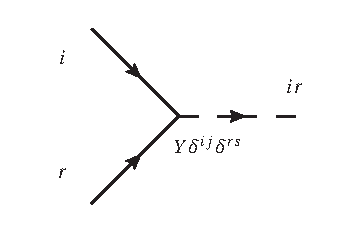
\includegraphics{abschnitte/QCDxdQCD/fig/Yukawa.eps}
 \caption{Möglicher Yukawa-Vertex in $SU(\Nc)\times SU(\Nd)$. Die Pfeile 
 zeigen dabei die Ladungserhaltung an.}
 \label{fig:QCDxdQCD:Yukawa_Majorana}
\end{figure}

    Berücksichtigt man gleichzeitig die Flavour-Quantenzahl, kann es insgesamt 
    $(\nfc \nfd \nsj)$ verschiedene Yukawa-Kopplungen geben. Eine 
    allgemeine Untersuchung ist also auch hier schwierig, da durch Änderungen 
    des Materieinhaltes auch die Anzahl der 
    Yukawa-Kopplungskonstanten gändert wird. Eine Möglichkeit dieses Problem 
    zu umgehen ist die Einführung von 
    Falvoursymmetrien, sodass für alle Yukawa-Terme nur 
    eine einzige Kopplungskonstante $Y$ verbleibt.
    In Abschnitt \ref{beta_QCDxdQCD} 
    entfallen solche Yukawa-Wechselwirkungen jedoch wieder, da $\nsj=0$ oder 
    $\nfd=0$ gewählt werden kann, ohne qualitativ unterschiedliche UV-Verhalten 
    zu verlieren. 
    
    Yukawa-Terme mit Dirac-artiger Lorentzstruktur, 
    \begin{equation}
     Y^{i,r,js} \psi^\dagger_i \xi_r \eta_{js} \, + \, 
     \text{ähnliche Terme} \quad ,
    \end{equation}
    sind in den gewählten Darstellungen nicht Eichinvariant. Hier besteht die 
    Möglichkeit, den dQCD-Sektor konjugiert 
    fundamental transformieren zu lassen, in der infinitesimalen 
    Transformation 
    \begin{equation}
     \xi_{r} \longrightarrow 
     \left(\mathbb{1}_{ru}-\i\delta^M \left(\widetilde{t}^M_{ru}\right)^*\right)
     \xi_{u} \quad , \quad
     \chi_{r} \,\,\, \text{analog}
     \quad ,
    \end{equation}
    wodurch wieder Yukawa-Kopplungen mit der Colour-Struktur von 
    \eqref{eq:QCDxdQCD:Yukawa_Struktur} erlaubt sind. Diese Möglichkeit würde 
    für die Eichkopplungen jedoch keinen Unterschied machen 
    und zu den selben $\beta$-Funktionen führen, sodass hier keine neuen 
    Phänomene im Vergleich zu \eqref{eq:QCDxdQCD:Yukawa_misch} zu erwarten sind.
    
  
      \item[3-Skalar-Kopplung:]
    Da die Fermionen und Skalare des QCD-, dQCD bzw. joint-Sektors jeweils 
    dieselben Transformationseigenschaften besitzen, können die Ergebnisse 
    \eqref{eq:QCDxdQCD:Yukawa_diagonal} und \eqref{eq:QCDxdQCD:Yukawa_Struktur} 
    für die Eichstruktur der 3-Skalar-Kopplungen übernommen werden. Es folgt, 
    dass die einzige Möglichkeit einer 3-Skalar-Kopplung mit einer nicht 
    veränderlichen Anzahl von Kopplungskonstanten $\lambda$
    \begin{equation}
     \mathcal{L}_\text{3-Skalar}= \lambda \phi_i \chi_r \eta_{ir}^* \hc
    \end{equation}
    ist. In \cite{Jones} schlägt Jones vor, 3-Skalar-Kopplungen durch diskrete 
    Symmetrien zu verbieten, Luo, Wang und Xiao zeigen in \cite{Luo_Wang_Xiao}, 
    dass 3-Skalar-Terme durch 4-Skalar-Terme mit einem unphysikalischen 
    Dummy-Feld beschrieben werden können.
    

     \item[4-Skalar-Kopplung:]
    Korrekturen durch 
    4-Skalar-Kopplungen tragen erst ab 3-Schleifen Ordnung zur $\beta$-Funktion 
    der Eichkopplungen bei \cite{quartic_scalar}, da in dieser Arbeit jedoch 
    nur 2-Schleifen $\beta$-Funktionen betrachtet werden, müssen sie nicht 
    berücksichtigt werden.
%     
    \end{description}
%     
%     
%   Aufgrund\cite{Ade:2015xua}